\documentclass{beamer}
 
\usepackage[utf8]{inputenc}
\usepackage{amsmath}
\usepackage{tabto}
\usepackage{graphicx}

 
%Information to be included in the title page:

\usetheme{Copenhagen}
\title[ADAM] %optional
{ADAM : A Method for Stochastic Optimization \\ in ICLR 2015 \\ By Diederik P. Kingma \hspace{1cm} Jimmy Lei Ba}
 
 
\author[Anshika,Razat] % (optional, for multiple authors)
{Anshika Chaurasia \and \\Razat Shanker}
 
\institute[VFU] % (optional)
{
  
  EE18MTECH11017\\
  EE18MTECH11016
 
 }
 
\date[VLC 2013] % (optional)
{4 Mar 2019}
 
 
\begin{document}
 
\frame{\titlepage}

\begin{frame}
\frametitle{Motivation}
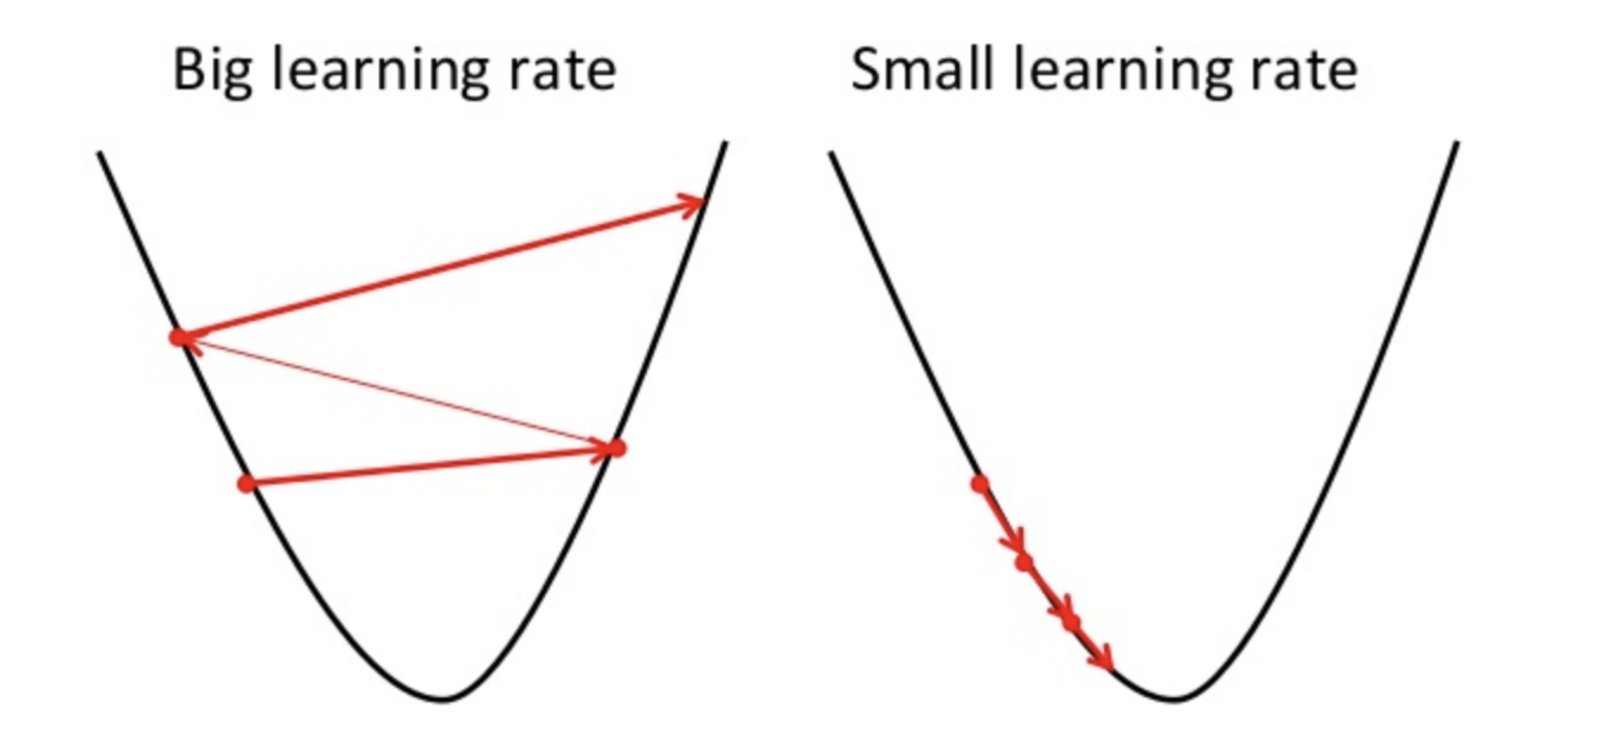
\includegraphics[width=9cm,height=5cm,angle=0]{Learning}
\begin{itemize}
    \item Learning rate affect model performance. 
    \item We want cost function sensitive to some directions in parameter space and insensitive to others
\end{itemize}
\end{frame}

\begin{frame}
 \frametitle{Related Work}
\begin{block}{AdaGrad}
Learning rate scaled by inverse of square of sum of all the previous squared values of the gradient
\end{block} 
\textbf{while } $\theta_{t}$ not converged \textbf{do} \\
\hspace{1cm} t $\leftarrow$ t + 1 \\
\hspace{1cm} g_{t} $\leftarrow \nabla_{\theta} f_{t}(\theta_{t-1})$ (get gradients w.r.t.         stochastic objective at \\ \hspace{1cm} timestep t) \\

\hspace{1cm} v_{t} $\leftarrow \ v_{t-1} + g_{t}^{2}$ (update biased     second  \\ \hspace{1cm} moment estimate ) \\

\hspace{1cm} \theta_{t} $\leftarrow \theta_{t-1} - \frac{\alpha}{\sqrt{v_{t}+\epsilon}}$ \odot g_{t} (update Parameter) \\
\textbf{end while}\\
\textbf{return } $\theta_{t}$ ( resulting parameter)
\end{frame}

\begin{frame}
 \frametitle{Related Work}
\begin{block}{RMSprop}
Uses an exponentially weighted moving average to discard history from the extreme past
\end{block}
\textbf{while } $\theta_{t}$ not converged \textbf{do} \\
\hspace{1cm} t $\leftarrow$ t + 1 \\
\hspace{1cm} g_{t} $\leftarrow \nabla_{\theta} f_{t}(\theta_{t-1})$ (get gradients w.r.t.         stochastic objective at \\ \hspace{1cm} timestep t) \\

\hspace{1cm} v_{t} $\leftarrow \ \beta_{1}v_{t-1} + (1 - \beta_{1})g_{t}^{2}$ (update biased     second \\ \hspace{1cm} moment estimate ) \\

\hspace{1cm} \theta_{t} $\leftarrow \theta_{t-1} - \frac{\alpha}{\sqrt{v_{t}+\epsilon}}$ \odot g_{t} (update Parameter) \\
\textbf{end while}\\
\textbf{return } $\theta_{t}$ ( resulting parameter)
\end{frame}

\begin{frame}
 \frametitle{Proposed Work}
\begin{block}{ADAM}
\begin{itemize}
    \item It is a combination of RMSprop and SGD with momentum. \\
    \item It uses the squared gradients to scale the learning rate like RMSprop\\
    \item It takes advantage of momentum by using moving average of the gradient like SGD with momentum
\end{itemize}
\end{block} 
\end{frame}

\begin{frame}
\frametitle{Algorithm}

$g_{t}^{2}$ indicates the element wise square g_{t} \odot g_{t} \\
\beta_{1} = 0.9 , $\beta_{2} = 0.999$ and \epsilon = 10^{-8} \\
\vspace{}

\textbf{Require : } \alpha : Stepsize \\
\textbf{Require : } $\beta_{1},\beta_{2} \hspace{1mm} \epsilon \hspace{1mm} $[0,1) :Exponential decay rates for the moment \\  estimates \\
\textbf{Require : } $f(\theta)$: Stochastic objective function with parameters \theta \\
\textbf{Require : } $\theta_{0}$ : Initial Parameter vector \\
m_{0}  $\leftarrow$ 0 (Initialize $1^{st}$ moment vector ) \\
v_{0}  $\leftarrow$ 0 (Initialize $2^{nd}$ moment vector ) \\
t  $\leftarrow$ 0 (initialize timestep) \\



\end{frame}
 
\begin{frame}
\frametitle{Algorithm}
\textbf{while } $\theta_{t}$ not converged \textbf{do} \\
\hspace{1cm} t $\leftarrow$ t + 1 \\
\hspace{1cm} g_{t} $\leftarrow \nabla_{\theta} f_{t}(\theta_{t-1})$ (get gradients w.r.t.         stochastic objective at \\ \hspace{1cm} timestep t) \\
\hspace{1cm} m_{t} $\leftarrow \beta_{1}m_{t-1} + (1 - \beta_{1}).g_{t}$ (update biased first     moment \\ \hspace{1cm} estimate ) \\
\hspace{1cm} v_{t} $\leftarrow \beta_{2}.v_{t-1} + (1 - \beta_{2}).g_{t}^{2}$ (update biased     second \\ \hspace{1cm} moment estimate ) \\
\hspace{1cm} m_{t}^{'} $\leftarrow m_{t}/(1 - \beta_{1}^{t})$ (compute bias-corrected first \\ \hspace{1cm} moment estimate ) \\
\hspace{1cm} v_{t}^{'} $\leftarrow v_{t}/(1 - \beta_{2}^{t})$ (compute bias-corrected second raw \\ \hspace{1cm} moment estimate ) \\
\hspace{1cm} \theta_{t} $\leftarrow \theta_{t-1} - \alpha .m_{t}^{'}/(\sqrt{v_{t}^{'}}+\epsilon)$ (update parameters) \\
\textbf{end while}\\
\textbf{return } $\theta_{t}$ ( resulting parameter)
\end{frame}
 
 \begin{frame}
 \frametitle{Experiment}

\begin{center}
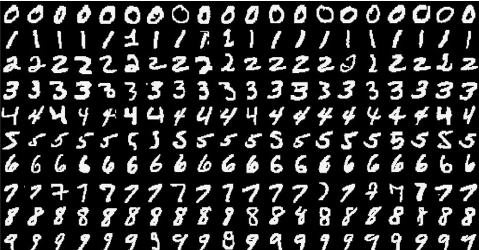
\includegraphics[width=9cm,height=6cm,angle=0]{mnist} \\
Fig :  MNIST Dataset    
\end{center}


\end{frame}
 
\begin{frame}
 \frametitle{Results}
 \begin{center}
 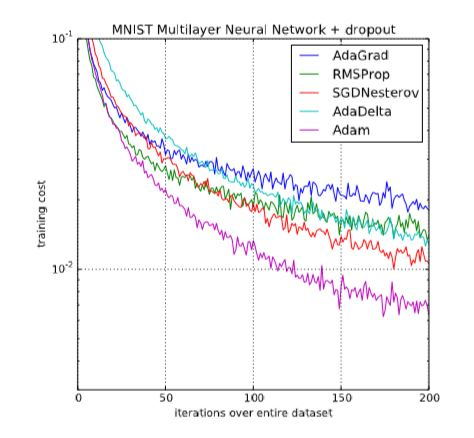
\includegraphics[width=7cm,height=5cm,angle=0]{mlp} \\
 Fig : Multilayer Neural Network on MNIST images
 \end{center}
\end{frame}

\begin{frame}{Why are neural networks non - convex ?}
 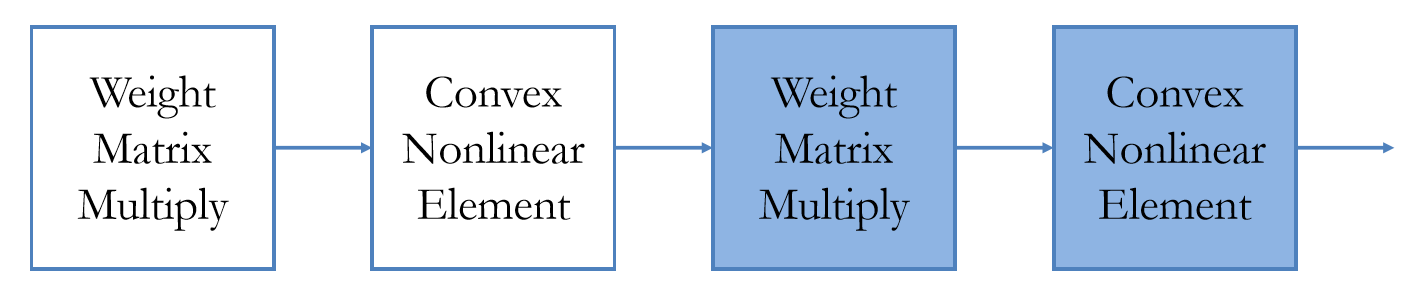
\includegraphics[width=12cm,height=3cm,angle=0]{nn}  \\
 \begin{itemize}
     \item composition of convex function is not convex
     \item Neural Networks are universal function approximators
     \item Convex functions can't approximate non - convex functions
 \end{itemize}
\end{frame}

\begin{frame}{Local Optimization of non convex functions}
    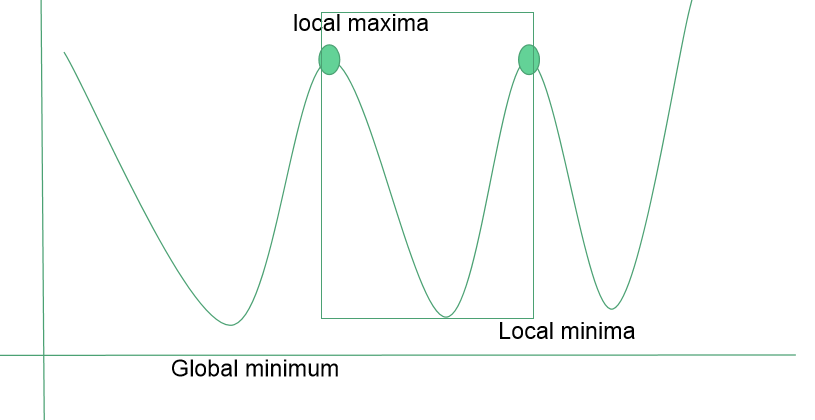
\includegraphics[width=11cm,height=7cm,angle=0]{nonconv}
\end{frame}

\begin{frame}
\frametitle{References}
[1] Duchi, John, Elad Hazan, and Yoram Singer. "Adaptive subgradient methods for online learning and stochastic optimization." Journal of Machine Learning Research 12.Jul (2011): 2121-2159. \\

[2] Sutskever, I., Martens, J., Dahl, G. E., & Hinton, G. E. (2013). On the importance of initialization and momentum in deep learning. ICML (3), 28(1139-1147), 5. \\

[3] Kingma, Diederik P., and Jimmy Ba. "Adam: A method for stochastic optimization." arXiv preprint arXiv:1412.6980 (2014).

\end{frame}

\end{document}
